% Roll Number 52, Reon Kurian

\textbf{\textcolor{LightMagenta}{Describe the concept of Density-based clustering and steps involved in DBSCAN Algorithm.(May 2019, Qn 18 (b))\hfill (Mark 6)}} \\[5pt]
In density-based clustering, clusters are defined as areas of higher density than the remainder of the data set. Objects in these sparse areas - that are required to separate clusters - are usually considered to be noise and border points. The most popular density-based clustering method is DBSCAN (Density-Based Spatial Clustering of Applications with Noise). K means clustering will fail to cluster based on density as it would cluster based on the distance to the nearest centroid. It would obtain different clusters in comparison to density based , Its fails to capture the complex density pattern in the data sets. 
Fig shows examples of cases where Density based clustering can be applied to capture the complex patterns.
\begin{figure}[htp]
    \centering
    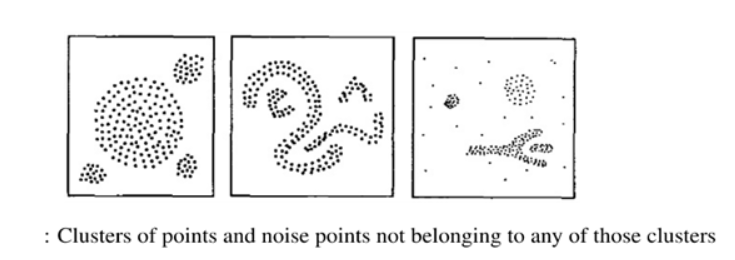
\includegraphics[width=10cm]{Images/A39_img1.png}
 \end{figure}

DBSCAN algorithm requires two parameters –

\begin{enumerate}
    \item eps :It defines the neighborhood around a data point i.e. if the distance between two points is lower or equal to ‘eps’ then they are considered as neighbors. If the eps value is chosen too small then large part of the data will be considered as outliers. If it is chosen very large then the clusters will merge and majority of the data points will be in the same clusters. One way to find the eps value is based on the k-distance graph.
    \item MinPts: Minimum number of neighbors (data points) within eps radius. Larger the dataset, the larger value of MinPts must be chosen. As a general rule, the minimum MinPts can be derived from the number of dimensions D in the dataset as, MinPts >= D+1. The minimum value of MinPts must be chosen at least 3.
\end{enumerate}
In this algorithm, we have 3 types of data points:(i)Core Point: A point is a core point if it has more than MinPts points within eps.
(ii)Border Point: A point which has fewer than MinPts within eps but it is in the neighbourhood of a core point.
(iii)Noise or outlier: A point which is not a core point or border point.


Steps involved in DBSCAN Algorithm:
\begin{enumerate}
    \item Find all the neighbor points within eps and identify the core points or visited with more than MinPts neighbors.
    \item For each core point if it is not already assigned to a cluster, create a new cluster.
    \item Find recursively all its density connected points and assign them to the same cluster as the core point.A point a and b are said to be density connected if there exist a point c which has a sufficient number of points in its neighbors and both the points a and b are within the eps distance. This is a chaining process. So, if b is neighbor of c, c is neighbor of d, d is neighbor of e, which in turn is neighbor of a implies that b is neighbor of a.

    \item 
Iterate through the remaining unvisited points in the dataset. Those points that do not belong to any cluster are noise.
\end{enumerate}






 				
